\documentclass[12pt, a4paper]{article}

\usepackage[utf8]{inputenc}
\usepackage[T2A]{fontenc}
\usepackage[russian]{babel}
\usepackage{graphicx}
\usepackage[footnotesize]{caption2}
\usepackage{indentfirst}
\usepackage{titlesec}
\usepackage[]{placeins}
\usepackage{multirow}
\usepackage{longtable}

\usepackage[left=3cm,right=1.5cm,top=2.0cm,bottom=2.0cm,bindingoffset=0cm]{geometry}
\usepackage{pdfpages}
\usepackage[onehalfspacing]{setspace}
\onehalfspacing

\renewcommand{\baselinestretch}{1.1}
\renewcommand{\baselinestretch}{1.5} %для печати с большим интервалом

\newcommand{\sectionbreak}{\clearpage}
\renewcommand{\labelenumii}{\arabic{enumi}.\arabic{enumii}.}



\begin{document}
\sloppy
	
\begin{titlepage}
\newpage
		
\begin{figure}[t]
	\centering
	
\includegraphics[width=0.4\textwidth]{img/mgu}
\end{figure}
		
\begin{center}
Московский государственный университет имени М.В. Ломоносова \\
Факультет вычислительной математики и кибернетики \\
Кафедра автоматизации вычислительных комплексов \\
\end{center}
		
\vspace{4em}
\begin{center}
\large
Ермакова Татьяна Ивановна
\end{center}
	
\begin{center}
\Large
\bfseries
Метод и средства передачи данных в реальном времени в программно-конфигурируемых сетях
\end{center}

\vspace{3em}
\begin{center}
\large
\textsc{
	магистерская диссертация
}
\end{center}

\vspace{5em}
\begin{flushright}
	\textbf{Научный руководитель:}\\
	к.ф.-м.н с.н.с\\
	В.В.Балашов\\
\end{flushright}%


\vspace{\fill}
\begin{center}
Москва 2019
\end{center}
		
\end{titlepage}

\section*{Аннотация}
В данной работе реализован предложенный автором подход к передаче данных в условиях реального времени в программно-конфигурируемых сетях (ПКС). Подход основан на схеме управления трафиком в ПКС, описанной в предыдущих работах автора, и предложенном в данной работе алгоритме реконфигурации систем виртуальных каналов. Алгоритм реконфигурации основан на жадных стратегиях и позволяет произвести восстановление работы системы после отказов, минимизируя время простоя и количество изменений в таблицах коммутации. Реализация подхода выполнена в виде программного средства, выполняющего функции мониторинга сети и её реконфигурации в случае возникновения отказов с использованием предложенных алгоритма и схемы. Программное средство представляет собой приложение для ПКС-контроллера RUNOS. Проведённое экспериментальное исследование продемонстрировало работоспособность предложенного подхода и входящего в него алгоритма реконфигурации в условиях реального времени.

\renewcommand{\contentsname}{Содержание}
\tableofcontents

\section*{Введение}
\addcontentsline{toc}{section}{Введение}
Специфика передачи данных в вычислительных системах реального времени (ВС РВ) заключается в повышенных требованиях к надежности и наличии жестких ограничений на время выполнения обмена сообщениями между абонентами. При построении ВС РВ предпочтение отдается коммутируемым средам обмена, которые в отличие от каналов вида точка-точка позволяют сократить число физических кабелей и гибко распределить пропускную способность.

Для избегания конфликтов между потоками данных в коммутируемых средах обмена используется механизм виртуальных каналов. Для удовлетворения потребностей ВС РВ при помощи этого механизма к виртуальным каналам предъявляются требования на ограничение следующих характеристик:
\begin{itemize}
	\item пропускной способности;
	\item задержки передачи данных;
	\item флуктуации задержки (джиттера).
\end{itemize}

Выполнение данных требований обеспечивается назначением виртуальным каналам ряда параметров, состав которых зависит от используемой схемы построения ВС РВ. Параметры виртуальных каналов в совокупности с их маршрутами образуют конфигурацию сети. Существуют следующие стандарты построения коммутируемых сетей ВС РВ на основе виртуальных каналов:
\begin{enumerate}
	\item Avionics Full Duplex Ethernet (AFDX) \cite{afdx}.
	\item FC-AE-ASM-RT на основе Fibre Channel \cite{fcaert}.
\end{enumerate}

Недостатком данных решений является статичность системы виртуальных каналов. Существующие стандарты предусматривают наличие ограниченного набора заранее заданных конфигураций, изменение которого невозможно в ходе работы ВС РВ. Переключение между такими конфигурациями не дает возможности гибко реагировать на отказы при работе системы.

Решением данной проблемы могут служить программно-конфигурируемые сети (ПКС) \cite{sdn}. ПКС является перспективным видом компьютерных сетей, главной особенностью которых являются широкие возможности реконфигурации. Использование ПКС для передачи данных в реальном времени даст возможность производить расчет и применение новых конфигураций сети в ходе работы системы. Это позволит перераспределять потоки данных при возникновении отказов или смене режима работы системы. На текущий момент не существует готовых решений, допускающих использование ПКС в составе ВС РВ при контроле полного состава параметров управления трафиком, принятых для сетей на основе виртуальных каналов.

Данная работа посвящена созданию методов и средств, позволяющих использовать ПКС в системах реального времени с учётом предъявляемых требований качества обслуживания и обеспечивать возможность реконфигурации сети в ходе работы системы.

\section{Постановка задачи}
Целью работы является разработка подхода к использованию программно-конфигурируемых сетей в составе вычислительных систем реального времени. В основу подхода положена ранее разработанная автором схема управления потоками данных в ПКС на основе виртуальных каналов \cite{vlsdn}. Для достижения этой цели должны быть решены следующие задачи:
\begin{enumerate}
	\item Разработка алгоритма динамической реконфигурации виртуальных каналов в ПКС.
	\item Реализация предложенного алгоритма в рамках приложения для контроллера ПКС, выполняющего функции мониторинга сети и её реконфигурации при выявлении отказов.
	\item Экспериментальное исследование полученного решения по критерию работоспособности в условиях реального времени.
\end{enumerate}

\section{Управление трафиком в ВС реального времени с использованием виртуальных каналов} \label{sec:scheme}
\subsection{Схема управления трафиком}
В основе подхода, описанного в \cite{vdovin} и используемого в сетях AFDX \cite{afdx}, FC-AE-ASM-RT \cite{fcaert}, а также в ранее предложенной автором схеме управления трафиком в ПКС, лежит согласованная работа оконечных систем (абонентов) и коммутаторов:
\begin{itemize}
	\item Оконечные системы при помощи планировщика обеспечивают корректную выдачу данных в сеть. Планировщик на каждой оконечной системе формирует трафик для виртуальных каналов и мультиплексирует их для выдачи на физическую линию.
	\item Коммутатор осуществляет контроль трафика при помощи алгоритма текущего ведра независимо для каждого виртуального канала. При превышении заданной пропускной способности кадры данного канала начинают сбрасываться.
\end{itemize}


Для алгоритма текущего ведра вводится ряд параметров виртуального канала:
\begin{itemize}
	\item BAG -- минимальный интервал времени вежду началами выдачи последовательных кадров на данном виртуальном канале.
	\item $L_{max}$ -- максимальная длина передаваемого кадра.
	\item $J_{max}$ -- джиттер, максимальный промежуток времени между началом временного слота и началом передачи кадра.
\end{itemize}

Для контроля трафика вводится кредит на количество передаваемых байт, максимальное значение которого равно $AC_{max} = L_{max}(1 + \frac{J_{max}}{BAG})$. Значение
кредита увеличивается с течением времени пропорционально величине $\frac{L_{max}}{BAG}$.

При поступлении кадра (или пакета) на коммутатор значение кредита уменьшается на его размер в случае, если этот размер не превосходит значения кредита. Иначе кадр (пакет) сбрасывается. Такая схема позволяет контролировать пропускную способность и джиттер. Работа алгоритма показана на рисунках~\ref{pic:scheme:nojit} и~\ref{pic:scheme:jit}.

\begin{figure}[h!]
	\centering
	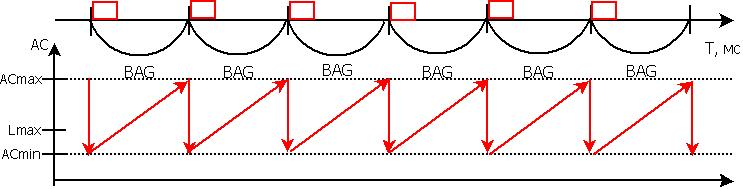
\includegraphics[width=0.80\textwidth]{img/nojit.png}
	\caption[russian]{Работа алгоритма текущего ведра при нулевом джиттере.}
	\label{pic:scheme:nojit}
\end{figure}

\begin{figure}[h!]
	\centering
	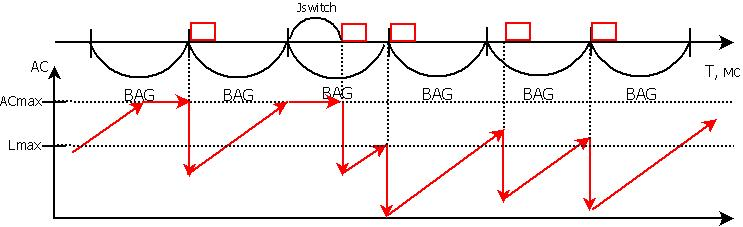
\includegraphics[width=0.80\textwidth]{img/jit.png}
	\caption{Работа алгоритма текущего ведра при ненулевом джиттере.}
	\label{pic:scheme:jit}
\end{figure}
\FloatBarrier

\subsection{Реализации схемы управления трафиком}
В данном разделе описываются индивидуальные особенности следующих схем управления трафиком:
\begin{itemize}
	\item Используемая в AFDX.
	\item Используемая в FC-AE-ASM-RT.
	\item Предложенная ранее автором схема управления трафиком в ПКС.
\end{itemize}

Стандарты AFDX и FC-AE-ASM-RT определяют построение сетей ВС РВ на основе виртуальных каналов. Маршрутизация в таких сетях производится коммутаторами при помощи статических таблиц, которые настраиваются заранее. Контроль трафика осуществляется с использованием алгоритма текущего ведра на уровне кадров в AFDX или пакетов в FC-AE-ASM-RT. Алгоритм контроля реализован в специализированных коммутаторах этих сетей.

В ПКС маршрутизация производится коммутаторами на основе динамических таблиц, задаваемых контроллером. Предложенная автором схема, описанная в \cite{vlsdn}, основывается на механизме meter-таблиц \cite{meter}, показанных на рисунке~\ref{pic:scheme:meter} и являющихся частью стандарта OpenFlow1.3 \cite{openflow}. Такие таблицы управляются контроллером и могут быть изменены в процессе работы системы. Каждая запись meter-таблицы задаёт измеритель, контролирующий скорость привязанных к нему потоков. Схема, по которой осуществляется данный контроль, не закреплена в стандарте и зависит от конкретных реализаций. 

\begin{figure}[h!]
	\centering
	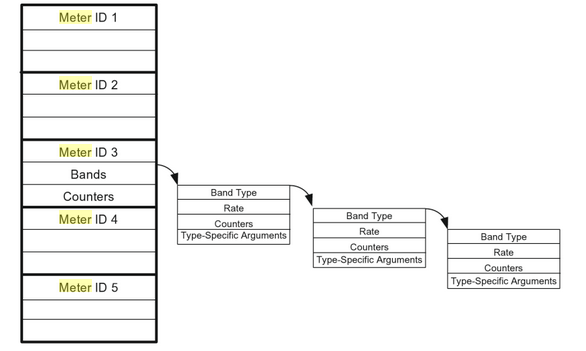
\includegraphics[width=0.80\textwidth]{img/meter.png}
	\caption{Структура meter-таблицы.}
	\label{pic:scheme:meter}
\end{figure}

Программный коммутатор Ofsoftswitch13 \cite{ofsoftswitch} реализует контроль трафика измерителями при помощи алгоритма текущего ведра и поэтому лег в основу предложенной автором схемы управления трафиком в ПКС.

Схема управления трафиком заключается в следующем:
\begin{itemize}
	\item Для каждого потока задается свой измеритель, на который средствами OpenFlow, посылается максимальное значение кредита и скорость его роста.
	\item Проверка допустимости трафика производится при помощи алгоритма текущего ведра отдельно для каждого потока на уровне пакетов.
\end{itemize}

\FloatBarrier
\subsection{Сравнение реализаций по критерию поддержки реконфигурируемости} \label{subsec:reconf}

Конфигурацией сети на основе виртуальных каналов назовем набор параметров виртуальных каналов в совокупности с их маршрутами. Каждой конфигурации соответствует набор таблиц маршрутизации, определяющих действия коммутаторов по передаче данных и контролю трафика в соответствии с данной конфигурацией.

Функционирование вычислительных систем реального времени может происходить в различных режимах. Для авиационных бортовых систем, к примеру, можно выделить режимы подготовки к полёту, взлёта, полёта и посадки. Каждому режиму присущи свои задачи и соответствующие им обмены данными. Поэтому каждому режиму соответствует своя конфигурация сети. Сбойными режимами работы системы назовём режимы, соответствующие предопределённой реакции на отказ или ряд отказов, возникающих в работе системы.

Динамическая реконфигурация сетей ВС РВ требуется в случаях:
\begin{enumerate}
	\item смены режимов работы;
	\item выхода из строя элементов сети (коммутаторов, портов, физических линий);
	\item выхода из строя вычислителей.
\end{enumerate}

Стандарт AFDX предусматривает наличие одной фиксированной таблицы маршрутизации на каждом коммутаторе. Такой набор таблиц маршрутизации соответствует единственной доступной в сети AFDX конфигурации. Для устранения последствий выхода из строя элементов системы используется полное дублирование сети. Альтернативные маршруты виртуальных каналов могут быть заложены в единственную конфигурацию сети. Однако такой подход требует резервирования пропускной способности под все маршруты виртуальных каналов, включая неиспользуемые, что ведёт к неэффективному использованию пропускной способности сети. Количество альтернативных маршрутов также ограничено доступной пропускной способностью в сети.

Стандарт FC-AE-ASM-RT имеет возможность поддерживать на коммутаторах несколько таблиц маршрутизации, задаваемых до начала работы системы. Это позволяет задать несколько конфигураций сети. Переход между такими конфигурациями осуществляется при помощи контроллера конфигураций. Им является дополнительная оконечная станция. При смене конфигурации контроллер сообщает коммутаторам сети идентификатор новой конфигурации. На каждом коммутаторе находится внутренняя оконечная станция, обрабатывающая информацию о смене конфигурации. Так как контроллером передается только идентификатор конфигурации, весь набор конфигураций должен быть заложен в коммутаторы до начала работы системы. На время процесса перехода, который может длиться до 40 мс, все коммуникации в системе временно приостанавливаются, так как происходит полная смена таблиц коммутации. Таким образом, процесс смены конфигурации нарушает циркуляцию трафика всех потоков данных системы. При использовании такой схемы существует возможность заложить несколько конфигураций сети, определяющих поведение системы при возникновении отказов.

В ПКС таблицы коммутаторов управляются контроллером при помощи сообщений, регламентируемых протоколом OpenFlow. В предложенной автором схеме модификация параметров виртуальных каналов производится сообщениями FlowMod и MeterMod протокола OpenFlow1.3. За счёт этого таблицы маршрутизации, равно как и meter-таблицы, могут быть изменены произвольным образом в ходе работы системы. Это позволяет создавать множество конфигураций, размер которого ограничен лишь возможностями физической среды передачи данных. Процесс изменения таблиц коммутации затрагивает не все содержащиеся в них правила. Это даёт возможность не нарушать движение трафика по виртуальным каналам, маршруты которых не проходили через отказавшие элементы сети. Для виртуальных каналов, пути следования которых были подвержены отказу, имеется возможность сохранить часть пакетов в случае совпадения участков старого и нового маршрутов. 

Как было показано выше, стандарт AFDX не поддерживает реконфигурацию в ходе работы системы. Возможностей же FC-AE-ASM-RT недостаточно для произведения гибкой реконфигурации, так как все сбойные режимы должны быть заранее заложены в систему. Для единичного отказа число таких режимов является достаточно большим и оценивается количеством физических элементов сети. Расчет всех случаев множественного отказа является ещё более нетривиальной задачей, а хранение всех таких конфигураций в памяти коммутаторов не представляется возможным. Использование ПКС в ВС РВ позволяет производить расчет и применение новой конфигурации сети непосредственно при возникновении отказа. Такой вариант реконфигурации позволяет системе частично продолжать функционировать даже в процессе перехода между конфигурациями. Всё это даёт возможность гибко реагировать на множественные отказы и восстанавливать работу системы в полном объеме в тех случаях, когда это позволяют физические ресурсы.


\section{Актуальность задачи}
Динамическая реконфигурация сети, как было показано в разделе~\ref{subsec:reconf}, востребована в ВС РВ. Возможность перераспределить потоки данных в ходе работы системы необходима при возникновении отказов или желании заложить несколько режимов работы в систему. Существующее решение на основе ПКС, предложенное в \cite{fakevlsdn}, не описывает схему контроля параметров качества обслуживания и представлено как альтернатива дублированию сети, обеспечивающая восстановление работы системы в случаях единичных отказов. 

В разделе \ref{sec:scheme} было продемонстрировано, что в ПКС имеются возможности для гибкой реконфигурации сети при соблюдении требований к качеству обслуживания, принятых в сетях ВС РВ. Для осуществления реконфигурации в случае возникновения отказов необходимо:
\begin{enumerate}
	\item Определить, в какой части сети произошел отказ.
	\item Произвести расчет новой конфигурации с учетом вышедших из строя элементов сети.
	\item Произвести переход на полученную конфигурацию.
\end{enumerate}

Данная работа посвящена алгоритму расчета новой конфигурации сети, а также его реализации в составе средства мониторинга и реконфигурации ПКС в условиях реального времени. Также в работе описан и реализован процесс локализации и идентификации отказов. Процедура смены конфигураций ранее была реализована и апробирована в рамках подтверждения работоспособности схемы управления трафиком в ПКС.

\section{Алгоритм реконфигурации виртуальных каналов} \label{sec:alg}
\subsection{Общая схема алгоритма}

В процессе разработки алгоритма реконфигурации был изучен ряд работ, посвященных построению маршрутов систем виртуальных каналов \cite{alg1}--\cite{vdovinalg}. Во всех перечисленных работах формирование конфигурации ведётся при помощи последовательного применения процедуры поиска маршрута к каждому из виртуальных каналов с использованием жадных стратегий. Статьи, посвященные не жадным стратегиям, рассмотрены не были из-за заведомо большого времени работы по этим стратегиям, несовместимого с функционированием в условиях реального времени. Также были изучены стандартные механизмы маршрутизации, принятые в ПКС \cite{algsdn}.

В основу предлагаемого алгоритма лёг описанный в работе \cite{vdovinalg} подход к построению систем виртуальных каналов для сетей AFDX. Однако этот подход не может быть позаимствован целиком, так как применяется для начальной инициализации сети и не удовлетворяет ограничениям, накладываемым в данной работе. Эти ограничения заключаются в том, что разрабатываемый алгоритм реконфигурации систем виртуальных каналов функционирует в условиях реального времени, а потому должен быть направлен на минимизацию:
\begin{itemize}
	\item времени расчёта новой конфигурации;
	\item времени применения новой конфигурации в сети, а значит и количества изменений в таблицах коммутации;
	\item числа пакетов, потерянных в процессе реконфигурации.
\end{itemize} 

Для достижения этих целей предлагаемый алгоритм разделён на два этапа -- базовый и дополнительный. На базовом этапе рассматриваются только те виртуальные каналы, которые необходимо переложить, так как они проходят через отказавшие элементы сети. В случае если невозможно произвести реконфигурацию, рассматривая только это множество виртуальных каналов, для восстановления работы сети выполняется дополнительный этап, на котором затрагивается более широкое множество виртуальных каналов. Общая схема алгоритма показана на рисунке~\ref{pic:algorithm}.

\begin{figure}[h!]
	\centering
	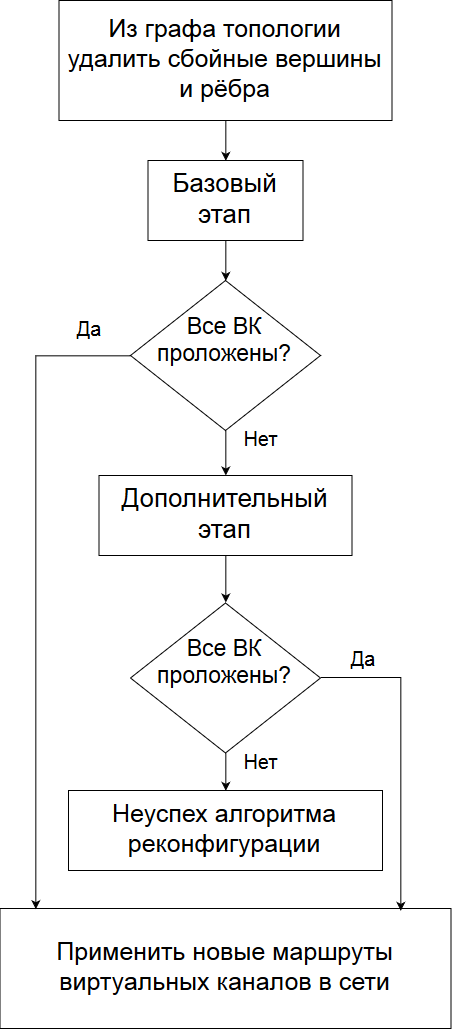
\includegraphics[width=0.50\textwidth]{img/alg.png}
	\caption{Общая схема алгоритма реконфигурации.}
	\label{pic:algorithm}
\end{figure}


Применение новых маршрутов в сети осуществляется только после успешного завершения работы алгоритма. Поведение приложения реконфигурации при неуспешном завершении алгоритма в рамках данной работы не рассматривается. Однако предполагается, что в этом случае будет предпринята попытка переложить часть виртуальных каналов в зависимости от критичности наличия соответствующих потоков данных для работы системы. 

\FloatBarrier

\subsection{Процедуры поиска нового маршрута виртуального канала} \label{subsec:procalg}
В основе каждого этапа алгоритма реконфигурации лежит поиск нового маршрута виртуального канала, который может осуществляться несколькими способами. Опишем эти способы прежде, чем приступить к описанию этапов алгоритма.

Введём обозначения:
\begin{itemize}
	\item $S$ -- узел-отправитель для данного виртуального канала.
	\item $R$ -- узел-получатель для данного виртуального канала.
	\item $Node_{S}$ – один из узлов, между которыми прервалась связь, ближний к $S$.
	\item $Node_{R}$ – один из узлов, между которыми прервалась связь, ближний к $R$.
\end{itemize}

Процедуры поиска нового маршрута виртуального канала основываются на жадных стратегиях. Их различие между собой заключается в глубине и скорости поиска. На базовом этапе алгоритма будет выполнен более быстрый вариант процедуры, так как цель базового этапа -- попытаться произвести реконфигурацию в как можно более короткий срок.

В основе обоих процедур лежат алгоритмы поиска кратчайшего пути, использующие вес ребра для определения длины пути. В качестве веса ребра в данной работе используется величина, обратная свободной пропускной способности соответствующей ему физической линии. Такое определение веса ребра позволяет выбирать путь с большим по сравнению с другими количеством оставшейся пропускной способности. 

Первый вариант процедуры поиска:
\begin{enumerate}
	\item Используя алгоритм Дейкстры \cite{dejkstra}, найти кратчайший путь между $Node_{S}$ и $R$.
	\item Добавить в него путь от $S$ к $Node_{S}$.
	\item Удалить циклы.
\end{enumerate}

Такая процедура поиска позволяет сохранить участок пути от $S$ к $Node_{S}$, когда это возможно. За счёт этого часть пакетов, отправляемых в процессе реконфигурации, не будет потеряна и будет перенаправлена по новому маршруту от $Node_{S}$ к $R$. Процедура направлена на минимизацию потерь пакетов, возникающих во время построения и применения новой конфигурации.

Второй вариант процедуры поиска:
\begin{enumerate}
	\item Используя алгоритм k-кратчайших путей \cite{kshort}, найти кратчайший путь между $S$ и $R$.
	\item Выбрать путь по критерию совпадения наибольшего числа узлов со старым маршрутом.
\end{enumerate}

Второй вариант процедуры даёт возможность найти большее количество альтернативных маршрутов. Для ограничения глубины поиска было выбрано значение $k = 3$. Ограничение на сохранение участка пути от $Node_{S}$ к $R$ снимается, но при этом выбор итогового маршрута зависит от исходного маршрута виртуального канала, что позволяет минимизировать число изменений в таблицах коммутации.

\subsection{Описание базового этапа алгоритма}

На данном этапе производится попытка найти новые маршруты для виртуальных каналов, проходивших через отказавшие элементы сети. Остальные виртуальные каналы при этом не затрагиваются. Такой подход при успешном завершении данного этапа позволяет произвести реконфигурацию с минимальными изменениями в сети. Ограниченный набор обрабатываемых виртуальных каналов и быстрая процедура поиска нового маршрута дают возможность минимизировать время работы базового этапа.

Обозначим за $(A)$ набор виртуальных каналов, проходивших через отказавший элемент сети. Пропускная способность вычисляется из параметров виртуального канала, описанных в разделе~\ref{sec:scheme} и равна:
$$bw = \frac{L_{max}}{BAG}$$

Базовый этап алгоритма реконфигурации:
\begin{enumerate}
	\item Для каждого виртуального канала из набора $(A)$ в порядке убывания пропускной способности выполнить:
	\begin{enumerate}
	\item Из графа, соответствующего текущей топологии сети, удалить все ребра, на которых не хватает пропускной способности для данного виртуального канала.
	\item Запустить первый вариант процедуры поиска нового маршрута виртуального канала, описанный в разделе~\ref{subsec:procalg}.
	\item В случае неуспеха перейти к пункту 2.
	\item Актуализировать значения пропускных способностей в графе сети с учётом построенного маршрута.
	\end{enumerate}
	\item Завершить этап.
\end{enumerate}

\subsection{Описание дополнительного этапа алгоритма}
Дополнительный этап запускается только в случае, если на базовом этапе не удалось построить новую конфигурацию сети. Целью данного этапа является осуществить реконфигурацию, несмотря на неуспех базового этапа, который показал, что нет возможности найти новые маршруты для виртуальных каналов из набора $(A)$ при существующем распределении оставшихся. Поэтому на данном этапе затрагивается более широкий набор виртуальных каналов, чем на базовом этапе. Помимо поиска новых маршрутов виртуальных каналов, проходивших через отказавшие элементы сети, также производится поиск новых маршрутов для некоторых из виртуальных каналов, старые маршруты которых не были затронуты отказом.

Пусть $bw_{max}$ -- максимальная пропускная способность виртуальных каналов из множества $(A)$.
Обозначим за $(B)$ набор виртуальных каналов, которые не входят в $(A)$ и пропускная способность которых не больше $bw_{max}$. Маршруты виртуальных каналов из набора $(B)$ не были затронуты отказом, однако для изменения ситуации в сети их маршруты на данном этапе будут пересчитаны. Использование такого набора $(B)$ позволяет не реконфигурировать виртуальные каналы с большой пропускной способностью, если это не необходимо.

На дополнительном этапе сначала осуществляется поиск новых маршрутов для всех виртуальных каналов из набора $(A)$. А затем аналогичный поиск для виртуальных каналов из набора $(B)$. При этом используется вторая процедура поиска из раздела~\ref{subsec:procalg}. Данная процедура направлена на выбор маршрута, переход на который минимизирует число изменений в сети , так как он наиболее приближен к старому маршруту. Поэтому совместный поиск новых маршрутов для наборов $(A)$ и $(B)$ в порядке убывания пропускных способностей входящих в них виртуальных каналов строил бы конфигурацию сети, слишком приближенную к существующей. Последовательный поиск новых маршрутов для виртуальных каналов сначала из набора $(A)$, а затем уже из набора $(B)$, позволяет изменить ситуацию в сети и найти новые маршруты для нарушенных виртуальных каналов. Более глубокая процедура поиска нового маршрута, используемая на данном этапе, также способствует вычислению доступной конфигурации сети. 


Дополнительный этап алгоритма реконфигурации:
\begin{enumerate}
	\item Для каждого виртуального канала из набора $(A)$ в порядке убывания пропускной способности выполнить:
	\begin{enumerate}
		\item Из графа, соответствующего текущей топологии сети, удалить все ребра, на которых не хватает пропускной способности для данного виртуального канала.
		\item Запустить второй вариант процедуры поиска нового маршрута виртуального канала, описанный в разделе~\ref{subsec:procalg}.
		\item В случае неуспеха перейти к пункту 3.
		\item Актуализировать значения пропускных способностей в графе сети с учётом построенного маршрута.
	\end{enumerate}
	\item Для каждого виртуального канала из набора $(B)$ в порядке убывания пропускной способности выполнить:
	\begin{enumerate}
		\item Из графа, соответствующего текущей топологии сети, удалить все ребра, на которых не хватает пропускной способности для данного виртуального канала.
		\item Запустить второй вариант процедуры поиска нового маршрута виртуального канала, описанный в разделе~\ref{subsec:procalg}.
		\item В случае неуспеха перейти к пункту 3.
		\item Актуализировать значения пропускных способностей в графе сети с учётом построенного маршрута.
	\end{enumerate}
	\item Завершить этап.
\end{enumerate}

\subsection{Теоретические свойства алгоритма}

В данном разделе дана оценка сложности и приведено обоснование завершимости предложенного алгоритма.

В основе обоих этапов лежат процедуры поиска, описанные в разделе~\ref{subsec:procalg}. В их основе в свою очередь лежат алгоритмы Дейкстры и k-кратчайших путей. Оценки сложностей этих алгоритмов равны $O(n^2)$ и $O(kn^3)$ соответственно, где $n$ -- число вершин в графе поиска. Данные оценки, как и факт завершимости указанных алгоритмов, могут быть найдены в \cite{dejkstra, kshort}. В разделе~\ref{subsec:procalg} обоснован выбор $k=3$. 

Введем обозначения:
\begin{itemize}
	\item $SW$ -- количество коммутаторов в сети;
	\item $VL$ -- количество виртуальных каналов;
\end{itemize}

В процедуре поиска маршрута виртуального канала участвует не более, чем $SW + 2$ узлов сети -- отправитель, получатель и в худшем случае все коммутаторы сети. Часть коммутаторов может не участвовать из-за отказов или исключения их из графа поиска по соображениям нехватки пропускных способностей на прилегающих к ним физических линиях. При этом процедура поиска на обоих этапах будет повторена не более, чем $VL$ раз, так как суммарный размер наборов $(A)$ и $(B)$ не превосходит $VL$.

Тогда оценка сложности для базового этапа равна $O(VL \ast (SW + 2)^2)$. Оценка сложности для дополнительного этапа -- $O(VL \ast 3(SW + 2)^3)$. Общая оценка сложности -- $O(VL(3(SW + 2)^3 + (SW + 2)^2))$. Алгоритм представляет собой повторение завершимых процедур не более, чем $2 \ast VL$ раз, что доказывает его завершимость.




\section{Структура и функции приложения реконфигурации}
\subsection{Назначение и структура приложения реконфигурации}

Приложение реконфигурации для ПКС-контролера, реализующего предлагаемый подход, должно:
\begin{itemize}
	\item реализовывать функции мониторинга для обнаружения и локализации отказов;
	\item реализовывать функции реконфигурации при возникновении отказов, а именно расчета новой конфигурации и её применения в сети;
	\item производить расчет новой конфигурации с использованием алгоритма, предложенного в разделе~\ref{sec:alg};
	\item применять изменения в сети на основе схемы, описанной в разделе~\ref{sec:scheme}.
\end{itemize}

Общая структура приложения реконфигурации, разработанного автором, показана на рисунке~\ref{pic:netcontrol}.

\begin{figure}[h!]
	\centering
	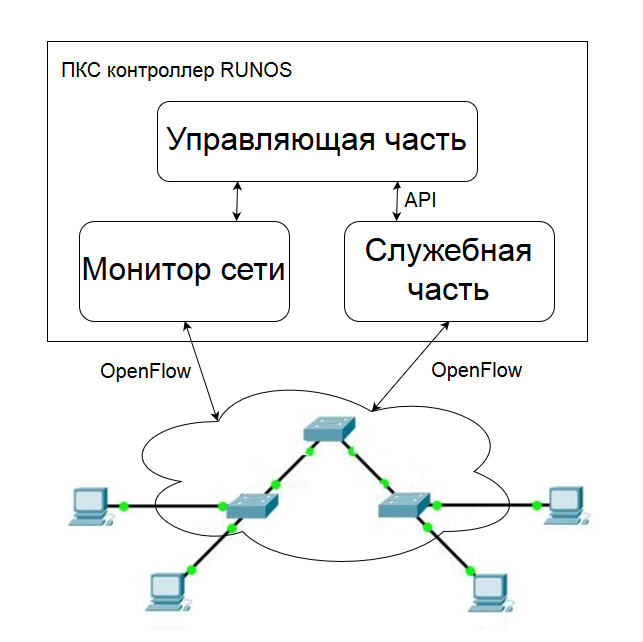
\includegraphics[width=0.90\textwidth]{img/netcontrol.png}
	\caption{Структура приложения реконфигурации.}
	\label{pic:netcontrol}
\end{figure}

\FloatBarrier
\subsection{Описание функций служебной части}
Служебная часть реализует в себе описанную в разделе~\ref{sec:scheme} схему управления трафиком в ПКС на основе виртуальных каналов.
 
Служебная часть должна предоставлять управляющей:
\begin{itemize}
	\item информацию о потоках данных, которыми обмениваются абоненты сети;
	\item информацию о проложенных в сети виртуальных каналах и их параметрах;
	\item интерфейс для добавления/удаления/модификации виртуальных каналов с определенными параметрами качества обслуживания.
\end{itemize}

\subsection{Описание функций управляющей части}
Управляющая часть реализует в себе описанный в разделе~\ref{sec:alg} алгоритм реконфигурации систем виртуальных каналов.

Управляющая часть:
\begin{itemize}
	\item отвечает за построение начальных маршрутов виртуальных каналов или загрузку готовых маршрутов, рассчитанных заранее другими средствами, например, \cite{vdovin};
	\item отвечает за построение новых маршрутов виртуальных каналов при отказах компонентов сети;
	\item использует API служебной части для применения новых маршрутов в сети после завершения работы алгоритма реконфигурации;
	\item использует информацию, полученную от монитора, для инициализации алгоритма реконфигурации.
\end{itemize}

\subsection{Описание функций монитора} \label{subsec:monitor}

Необходимо осуществлять мониторинг следующих компонентов сети:
\begin{enumerate}
	\item Коммутаторов.
	\item Физических линий связи.
	\item Оконечных систем.
\end{enumerate}

Мониторинг состояния коммутаторов и физических линий между коммутаторами производится стандартным для ПКС способом, описанным в \cite{monitor1, monitor2}. Ниже приведено краткое описание процедур мониторинга. В силу специфики задачи, а именно необходимости совместной работы отправителей и коммутаторов, оконечные системы должны функционировать по предопределенной схеме. Особенности их функционирования задаются в момент проектирования системы. Поэтому на них может быть возложена функция отправки диагностических пакетов. Это позволяет использовать схему мониторинга состояния оконечных систем, в которой нагрузки на сеть данных ниже в сравнении с со стандартной схемой.

Все процессы мониторинга выполняются периодически. Выбираемый период влияет на количество служебных пакетов в сети и на скорость реагирования при возникновении отказов. Было выбрано значение 10 мс, так как оно является соразмерным допустимому времени простоя ВС РВ, указанному в разделе \ref{subsec:reconf}. Такой период значительно меньше принятого в ПКС, что ведёт к увеличению нагрузки на управляющую сеть и сеть данных. При этом не относящаяся к мониторингу нагрузка на управляющую сеть в предлагаемом подходе весомо ниже. Большую часть времени система работает в проактивном режиме, установка правил происходит только в период инициализации и реконфигурации системы. Трафик мониторинга, как правило, является единственным трафиком в управляющей сети и потому возможно увеличение его объема. В сети данных часть пропускной способности должна быть выделена под диагностические пакеты. Это учитывается при конфигурации системы и распределении потоков данных.

Мониторинг состояния коммутаторов производится на уровне OpenFlow при помощи сообщений EchoReq и EchoRes. Раз в период коммутатор и контроллер обмениваются ими для подтверждения работоспособности друг друга.

Мониторинг состояния оконечных систем производится по следующей схеме:
\begin{enumerate}
	\item Оконечная система раз в период посылает пакет на ближайшие коммутаторы.
	\item На коммутаторах инициируется сообщение Packet-in, сообщающее контроллеру о поступлении неизвестного пакета.
	\item Контроллер, не получив раз в период ни одного Packet-in, в котором в поле отправителя содержится идентификатор данной оконечной системы, считает её отключённой.
\end{enumerate}


Процедуру мониторинга состояния физических линий можно разделить на две составляющие: 
\begin{itemize}
	\item мониторинг линий между коммутаторами;
	\item мониторинг линий между коммутаторами и оконечными системами.
\end{itemize}

Физическая линия считается вышедшей из строя в случае если с коммутатора поступило сообщение, свидетельствующее об отключении соответствующего порта. В рамках OpenFlow для этого используется сообщение PortStatus, его отправка инициируется самим коммутатором при изменении статуса порта.

Мониторинг линии между коммутаторами осуществляется на основе протокола Link Layer Discovery Protocol (LLDP), описанного в \cite{monitor2}, следующим образом:
\begin{enumerate}
	\item Контроллер отправляет инкапсулированный в Packet-out LLDP-пакет на соответствующий порт коммутатора. В Packet-out содержится информация о пересылке LLDP-пакета по исследуемой физической линии.
	\item Коммутатор отправляет LLDP-пакет по линии на другой коммутатор.
	\item Второй коммутатор, получив LLDP-пакет, инкапсулирует его в Packet-In и отправляет контроллеру.
	\item Получив обратно пакет, контроллер делает вывод о живости физической линии.
\end{enumerate}

Мониторинг линий между коммутаторами и оконечными системами производится совместно с мониторингом самих оконечных систем. Разница заключается в том, что каждый Packet-in отвечает за свою физическую линию.

Монитор сети реализует описанную схему мониторинга, а также:
\begin{itemize}
	\item отвечает за построение начальной топологии сети;
	\item сообщает управляющей части о выходе из строя компонентов сети.
\end{itemize}

\section{Программная реализация}
\subsection{Выбор базового программного обеспечения сети}

В данном разделе обосновывается выбор коммутаторов и контроллера, используемых в предлагаемом подходе и проведенных исследованиях.

Выбор коммутаторов основывается на используемой схеме управления трафиком. При этом к коммутаторам предъявляются следующие требования:
\begin{itemize}
	\item Поддержка механизма meter-таблиц.
	\item Поддержка OpenFlow не ниже 1.3.
	\item Реализация механизма meter-таблиц должна основываться на алгоритме текущего ведра.
\end{itemize}

Корректность схемы управления трафиком в ПКС с использованием программного коммутатора Ofsoftswitch13 \cite{ofsoftswitch} была подтверждена в предыдущих работах автора. Поэтому выбор сделан в его пользу.

Выбор контроллера обусловлен следующими критериями:
\begin{itemize}
	\item Язык реализации С++, который обеспечивает более детерминированное по сравнению с другими языками программирования время работы. Обоснование этому может быть найдено в \cite{cpp}.
	\item Поддержка OpenFlow версии не ниже 1.3
	\item Наличие активной команды разработчиков.
\end{itemize}

Были рассмотрены следующие варианты контроллеров, реализованных на C++: NOX \cite{nox} и RUNOS \cite{runos}. Контроллер NOX больше не поддерживается разработчиками, тогда как RUNOS активно развивается, поэтому выбор был сделан в пользу второго.

\subsection{Структура программного средства}
Диаграмма, отражающая основные программные компоненты разработанного приложения реконфигурации, показана на рисунке~\ref{pic:classes}. Реализация выполнена на языке C++.

\begin{figure}[h!]
	\centering
	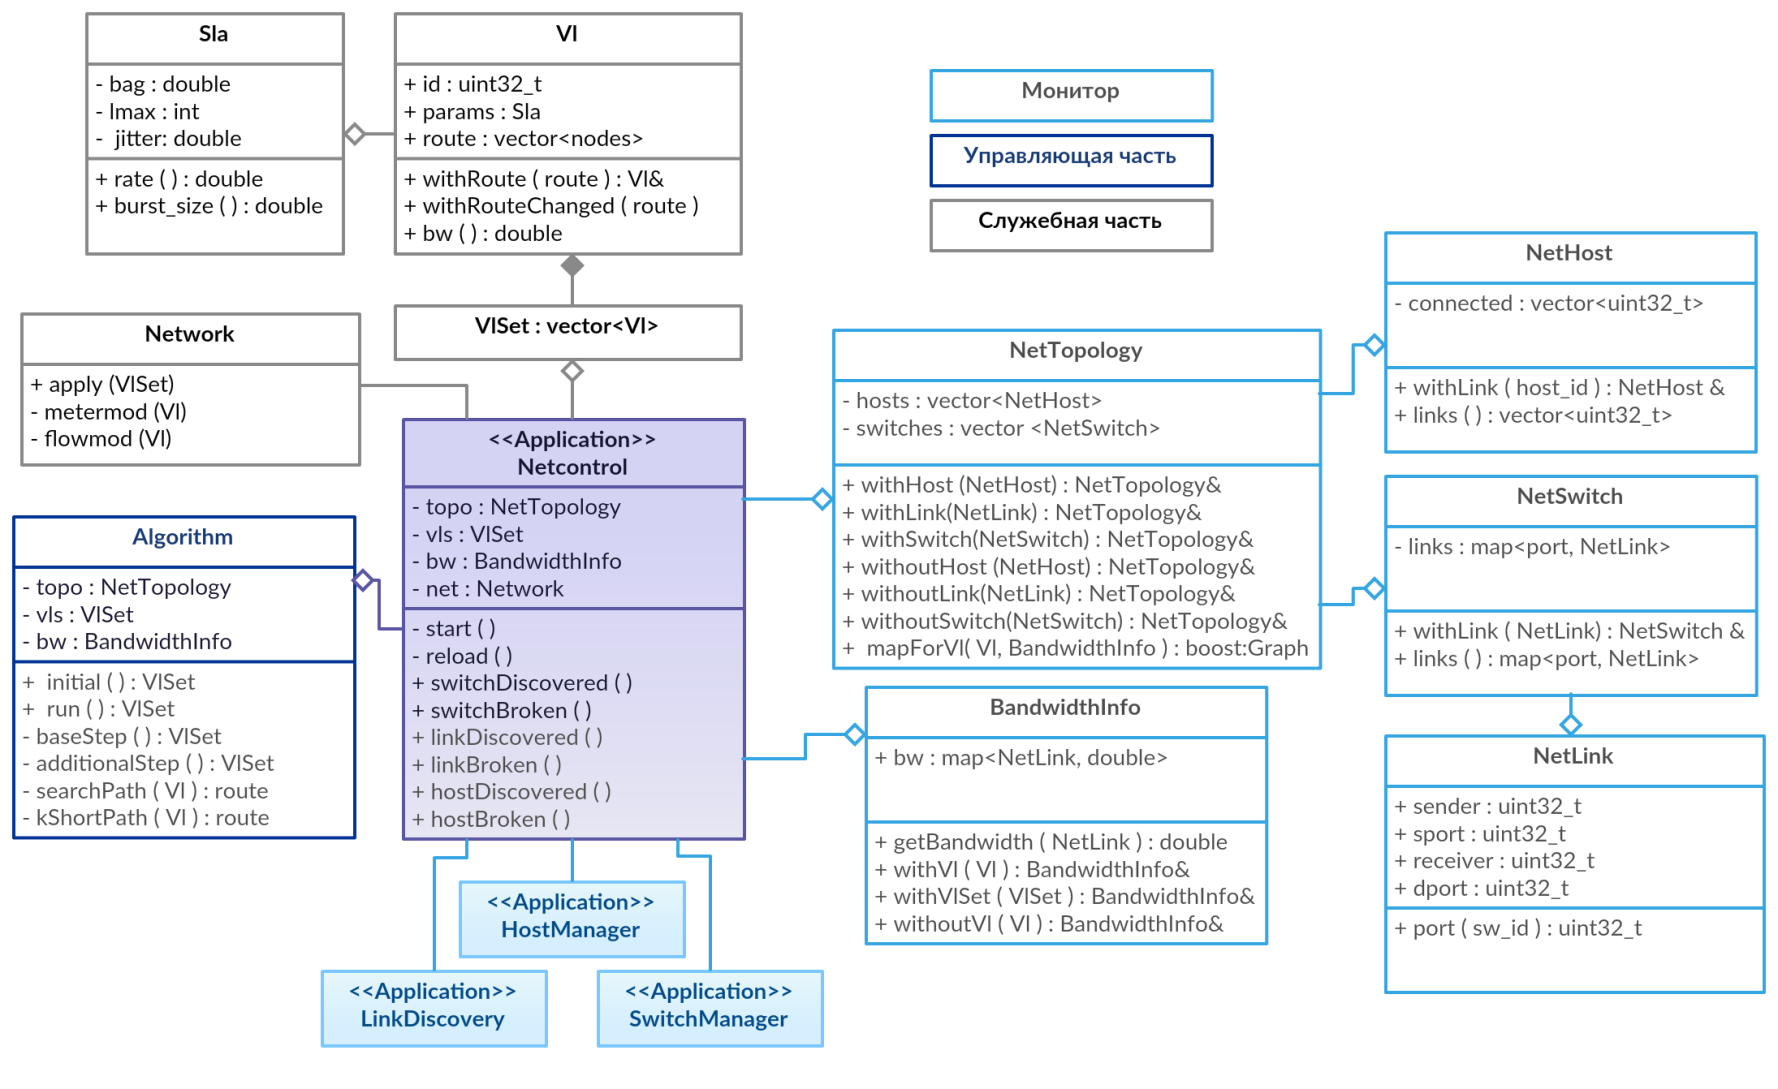
\includegraphics[width=1.0\textwidth]{img/classes.png}
	\caption{Основные классы программной реализации.}
	\label{pic:classes}
\end{figure}


Основные программные компоненты служебной части:
\begin{itemize}
	\item Sla -- класс характеристик виртуальных каналов.
	\item Vl -- класс, отвечающий за хранение параметров виртуальных каналов (включая их маршруты).
	\item VlSet -- набор виртуальных каналов.
	\item Network -- интерфейс для применения настроек виртуальных каналов. Формирует набор сообщений для применения соответствующих параметров и маршрутов в сети.
\end{itemize}

Основные программные компоненты управляющей части:
\begin{itemize}
	\item Netcontrol -- класс, отвечающий за запуск алгоритма реконфигурации и обработку данных, полученных от монитора. Является классом приложения Runos.
	\item Algorithm -- класс, реализующий алгоритмы построения маршрутов виртуальных каналов.
\end{itemize}

Основные программные компоненты монитора:
\begin{itemize}
	\item NetTopology -- класс, отображающий текущее состояние топологии сети. Использует вспомогательные классы NetLink, NetSwitch и NetHost для хранения информации о каналах, коммутаторах и абонентах соответственно.
	\item BandwidthInfo -- хранит текущую доступную на физических каналах пропускную способность. Начальные значения задаются в конфигурации приложения.
	\item HostManager -- приложение Runos, анализирующее состояние абонентов.
	\item SwitchManager -- приложение Runos, анализирующее состояние коммутаторов.
	\item LinkDiscovery -- приложение Runos, анализирующее состояние физических каналов.
\end{itemize}

Из перечисленных компонентов монитора компоненты SwitchManager и LinkDiscovery представляют собой стандартные приложения контроллера Runos, в которые внесены незначительные модификации. Остальные компоненты полностью реализованы автором работы. 

\section{Экспериментальное исследование}
\subsection{Цель исследования}
Целью исследования является анализ характеристик и подтверждение работоспособности в реальном времени предложенного в работе алгоритма реконфигурации виртуальных каналов, предназначенного для использования в рамках описанного подхода к передаче данных в ПКС в условиях реального времени. Для достижения поставленной цели необходимо:
\begin{itemize}
	\item провести исследование свойств алгоритма на различных классах входных данных; 
	\item провести апробацию работы алгоритма в составе приложения, реализующего функции реконфигурации и мониторинга;
	\item провести комплексную апробацию предлагаемого подхода передачи данных в условиях реального времени в ПКС.
\end{itemize}

Свойства алгоритма, подлежащие исследованию:
\begin{itemize}
	\item успешность и этап завершения;
	\item скорость работы.
\end{itemize}

Изучаемые в рамках апробации подхода характеристики системы:
\begin{itemize}
	\item успешность восстановления трафика в сети после завершения работы алгоритма реконфигурации;
	\item скорость применения изменений в сети;
	\item характеристики качества обслуживания для трафика абонентов (задержка и джиттер) после завершения реконфигурации.
\end{itemize}

\subsection{Классы исходных данных}
Параметры для формирования классов данных:
\begin{enumerate}
	\item Распределение виртуальных каналов по пропускным способностям.
	\item Общая загруженность сети.
	\item Топология сети.
\end{enumerate}

Расчёт пропускной способности виртуального канала производится в соответствии с формулой:
$$bw = \frac{L_{max}}{BAG}$$

Выделим типы виртуальных каналов в зависимости от пропускной способности:
\begin{itemize}
	\item легковесные ($bw=k$);
	\item средние ($bw=2k$);
	\item тяжёлые ($bw=4k$).
\end{itemize}

Величина $L_{max}$ для ВС РВ, как правило, составляет 1000 байт. Значение величины ${BAG}$ лежит в диапазоне 1-128 мс. Величина $k = \frac{L_{max}}{BAG}$, так как она отражает пропускную способность виртуального канала. Таким образом, $k$ выбрано равным 8 Мбит/c.

Классы исходных данных, сформированные на основе процентного содержания виртуальных каналов каждого типа, показаны в таблице~\ref{table:bwclass}. Данные классы выбраны для исследования случаев преобладания каждого из типов виртуальных каналов. Распределение пропускных способностей виртуальных каналов влияет на работу алгоритма, так как поиск альтернативных маршрутов виртуальных каналов затрудняется с ростом их пропускной способности.

\begin{table}[h]
	\caption{Классы данных на основе пропускной способности виртуальных каналов}
	\label{table:bwclass}
\begin{center}
\begin{tabular}{|c|c|c|c|}
\hline
	 Класс данных& Легковесные & Средние & Тяжёлые\\
\hline
	B1 & 90\% & 7\% & 3\% \\
\hline
 B2 & 10\% & 80\% & 10\% \\
\hline
	B3 & 33\% & 34\% & 33\% \\
\hline
	B4 & 5\% & 15\% & 80\% \\
\hline
\end{tabular}
\end{center}
\end{table}

Расчёт общей загруженности сети производится при помощи формулы, отражающей загрузку физических линий в зависимости от количества маршрутов виртуальных каналов, которые могут быть проложены через данную линию. Данный расчёт производится на этапе формирования исходных наборов данных при помощи разработанного автором вспомогательного средства на языке Python. Средство использует алгоритм k-кратчайших путей для поиска потенциальных маршрутов виртуальных каналов. Такой расчёт загруженности сети используется исключительно на этапе экспериментального исследования и не является частью представленного в работе алгоритма реконфигурации.

Для графа сети, в котором ребра соответствуют физическим линиям, введём вес ребра $e$:
$$p_{e} = \sum_{vl}\frac{bw_{vl} \ast k_{vl_e}}{k_{vl}}$$
где 
\begin{itemize}
	\item $vl$ -- множество виртуальных каналов;
	\item $bw_{vl}$ -- пропускная способность виртуального канала;
	\item $k_{vl_e}$ -- число кратчайших путей, построенных для данного канала, проходящих через это ребро;
	\item $k_{vl}$ -- количество найденных кратчайших путей для данного виртуального канала.
\end{itemize}

Тогда общая загруженность сети определяется формулой:
$$p = \max_{e}\frac{p_{e}}{bw_{e}}$$

где $bw_{e}$ -- пропускная способность физической линии.

Два класса исходных данных, формирующиеся на основе данного параметра, показаны в таблице~\ref{table:loadclass}. Общая загруженность сети влияет на работу исследуемого алгоритма. С ростом загруженности возрастает сложность поиска альтернативных маршрутов для виртуальных каналов. 

\begin{table}[h]
	\caption{Классы данных на основе загруженности сети}
	\label{table:loadclass}
\begin{center}
\begin{tabular}{|c|c|}
\hline
	Класс данных & Загруженность сети ($p$)\\
\hline
	L1 & 60\% \\
\hline
	L2 & 80\% \\
\hline
\end{tabular}
\end{center}
\end{table}

Для апробации работы приложения при выходе из строя различных элементов сети и демонстрации множества вариантов поиска альтернативного маршрута было выбрано три топологии:
\begin{enumerate}
	\item <<Ромб>> (рисунок~\ref{pic:4node}).
	\item <<Двойное резервирование>> (рисунок~\ref{pic:double}).
	\item <<Ассиметрия>> (рисунок~\ref{pic:5node}).
\end{enumerate}

\begin{figure}[h!]
	\centering
	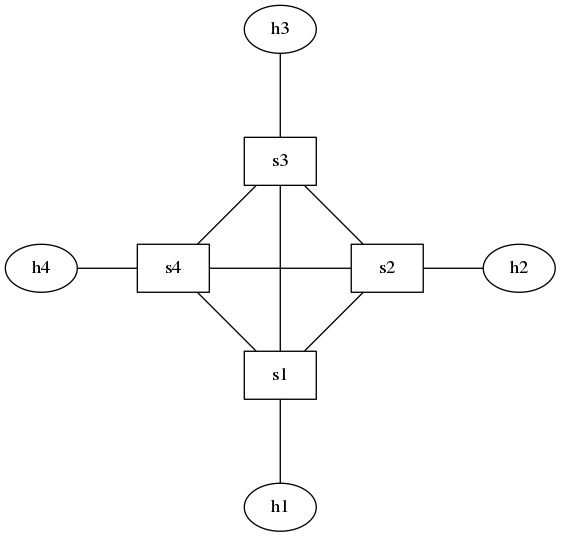
\includegraphics[width=0.40\textwidth]{img/4node.png}
	\caption{Топология <<Ромб>>.}
	\label{pic:4node}
\end{figure}

\begin{figure}[h!]
	\centering
	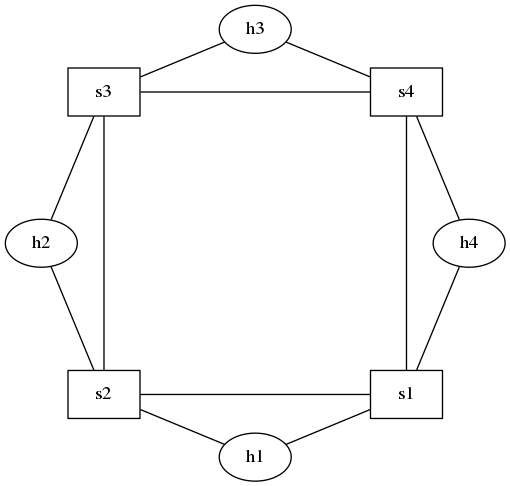
\includegraphics[width=0.40\textwidth]{img/double.png}
	\caption[russian]{Топология <<Двойное резервирование>>.}
	\label{pic:double}
\end{figure}

\begin{figure}[h!]
	\centering
	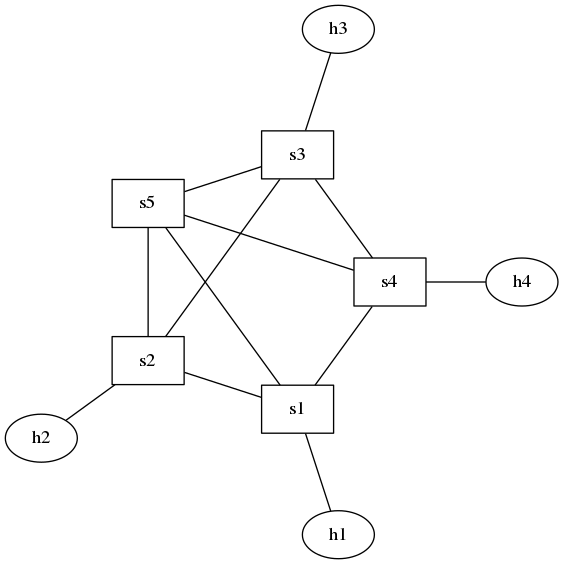
\includegraphics[width=0.40\textwidth]{img/5node.png}
	\caption{Топология <<Ассиметрия>>.}
	\label{pic:5node}
\end{figure}

В исследовании используется рекомендованное экспертами в области вычислительных реального времени число виртуальных каналов равное 100.
\FloatBarrier

Каждый набор данных, используемый в исследовании и апробации характеризуется принадлежностью к:
\begin{enumerate}
	\item одному из классов B1-B4, указанных в таблице~\ref{table:bwclass};
	\item одному из классов L1-L2, указанных в таблице~\ref{table:loadclass};
	\item одной из перечисленных выше топологий;
\end{enumerate}



\subsection{Накладываемые ограничения} \label{subsec:limits}
Процесс реконфигурации сети влечёт за собой потери пакетов, увеличение задержек и джиттеров. Чем быстрее будет производится смена конфигурации, тем меньшее воздействие этот процесс окажет на трафик абонентов бортовой системы. В рамках данного экспериментального исследования будем опираться на временные ограничения, принятые в вычислительных системах реального времени. Как упоминалось в разделе~\ref{sec:scheme}, в сетях FC-AE-ASM-RT на смену конфигурации отводится 40мс. При этом будем учитывать оценки на время, прошедшее с момента отправки последнего управляющего правила до момента его применения в таблице коммутации. С учетом небольших расстояний и низкой общей загруженности управляющей сети используем оценку в 10 мс. Также учтём, что выбранный в разделе~\ref{subsec:monitor} период обнаружения отказов равен 10 мс.

С учётом вышесказанного в качестве итогового времени, отводимого на реконфигурацию примем 20 мс. За это время с использованием предлагаемого алгоритма должны быть рассчитаны новые маршруты виртуальных каналов, а также сформированы и отправлены все управляющие пакеты для соответствующих изменений в таблицах коммутации.

\subsection{Исследование свойств алгоритма}
\subsubsection{Методика исследования}
Исследование свойств алгоритма производится по следующей схеме:
\begin{enumerate}
	\item Для каждого класса данных генерируется соответствующие ему наборы виртуальных каналов. Для наборов различаются периоды отправки пакетов, их размеры и распределения потоков данных между абонентами.
	\item Для каждого набора виртуальных каналов:
	\begin{enumerate}
		\item Запускается приложение, содержащее алгоритм реконфигурации.
		\item Разработанным программным средством выполняется построение начальных маршрутов виртуальных каналов.
		\item Собирается статистика по количеству виртуальных каналов, проходящих через каждый элемент сети.
		\item Выбирается элемент сети, через который проходит наибольшее число виртуальных каналов, и имитируется его отказ.
		\item Отказ инициирует запуск алгоритма реконфигурации.
		\item По завершении алгоритм выдаёт информацию об успешности и этапе завершения, а также о времени работы.
	\end{enumerate}
\end{enumerate}

Предполагается, что время работы алгоритма занимает не более 70\% от всего времени, заложенного на реконфигурацию, то есть не более 14 мс. По полученным характеристикам делается вывод о возможности использования алгоритма в рамках подхода к передаче данных в реальном времени. В результаты выносятся максимальные времена работы алгоритма, достигнутые на каждом из классов данных.
 
\subsubsection{Результаты}
Характеристики компьютера, на котором производилось исследование:
\begin{itemize}
	\item Процессор -- Intel Core i7, тактовая частота 1.90 ГГц.
	\item Оперативная память -- 4 ГБ.
\end{itemize}

Результаты исследования свойств алгоритма реконфигурации виртуальных каналов приведены в приложении A (см. таблицу A1).

Максимальное время работы алгоритма – 6.028 мс. Данные показатели времени достигаются, если алгоритм вынужден выполнить дополнительный этап. Следует отметить, что выполнение дополнительного этапа произошло в 28\% случаев. Как правило, алгоритм завершает работу на базовом этапе. При таком варианте выполнения время завершения алгоритма не превышает 3 мс. Дополнительный этап выполняется при высокой загруженности сети и при наличии большого количества виртуальных каналов с большой пропускной способностью (классы B3-B4 и L2). Время работы алгоритма, не превысило 35\% от времени, отведённого на реконфигурацию. То, как данная величина соотносится со временем, затрачиваемым на применение полученных изменений в сети, будет продемонстрировано в разделе~\ref{subsec:approbation}.

\begin{figure}[h!]
	\centering
	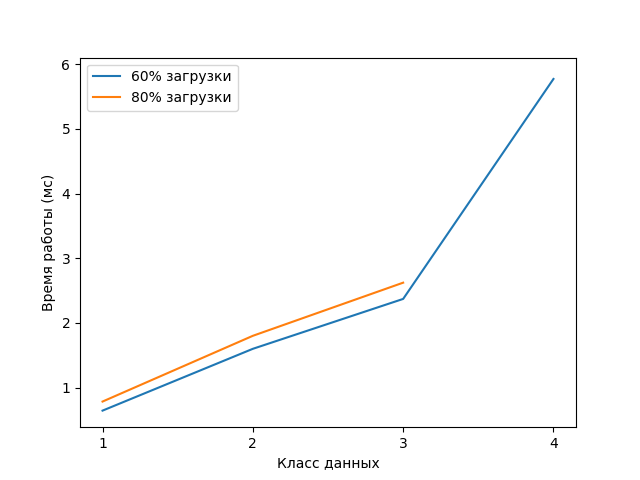
\includegraphics[width=0.60\textwidth]{img/5node_res.png}
	\caption{Работа алгоритма при выходе из строя линии в топологии <<Ассиметрия>>.}
	\label{pic:5node_res}
\end{figure}

\begin{figure}[h!]
	\centering
	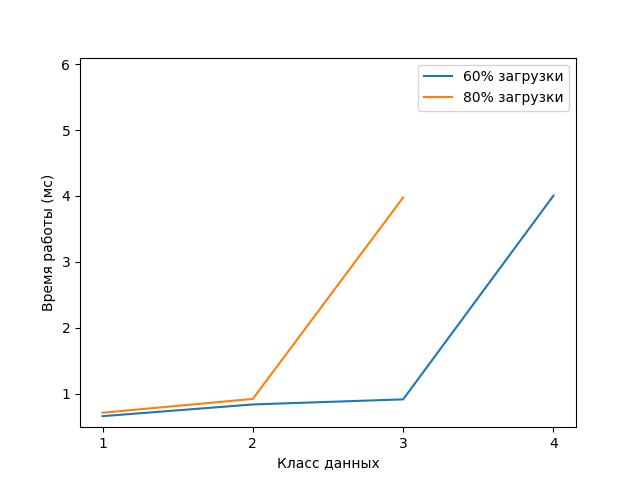
\includegraphics[width=0.60\textwidth]{img/4node_res.png}
	\caption{Работа алгоритма при выходе из строя линии в топологии <<Ромб>>.}
	\label{pic:4node_res}
\end{figure}

\begin{figure}[h!]
	\centering
	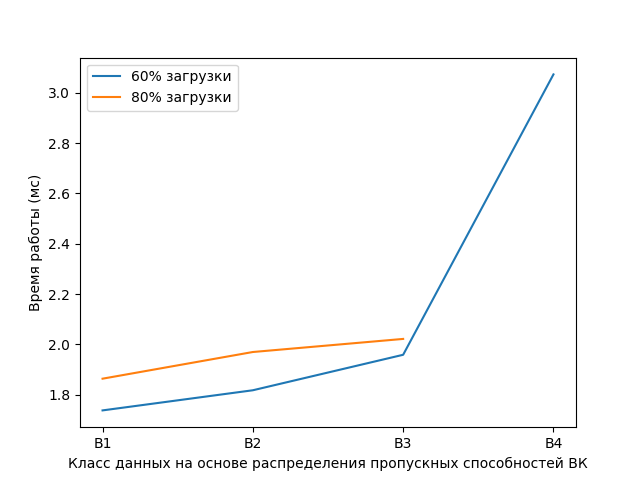
\includegraphics[width=0.60\textwidth]{img/double_res.png}
	\caption{Работа алгоритма при выходе из строя линии в топологии <<Двойное резервирование>>.}
	\label{pic:double_res}
\end{figure}


Алгоритм не смог построить новую систему виртуальных каналов при отказе линий в случае 80\% загрузки сети и большого количества виртуальных каналов с высокой пропускной способностью. Это объясняется тем, что на дополнительном этапе новые пути некоторых виртуальных каналов были слишком приближены к старым путям, то есть для них существовал альтернативный путь, требующий большего количества изменений в сети. Выбор такого пути изменил бы ситуацию в сети и позволил бы проложить оставшиеся виртуальные каналы.

\begin{figure}[h!]
	\centering
	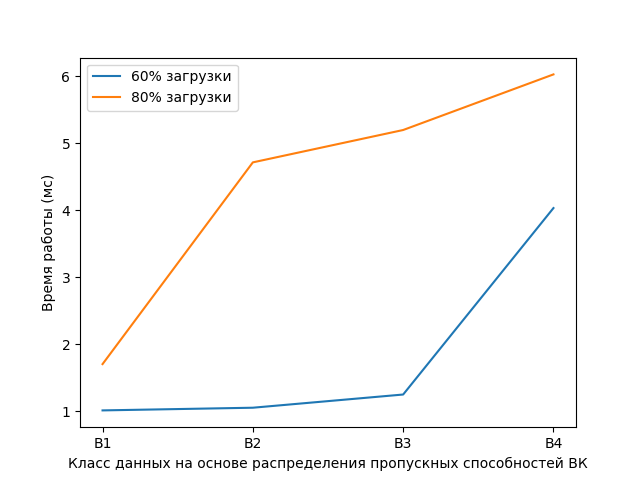
\includegraphics[width=0.60\textwidth]{img/5node_res_sw.png}
	\caption{Работа алгоритма при выходе из строя коммутатора в топологии <<Ассиметрия>>.}
	\label{pic:5node_res_sw}
\end{figure}

\begin{figure}[h!]
	\centering
	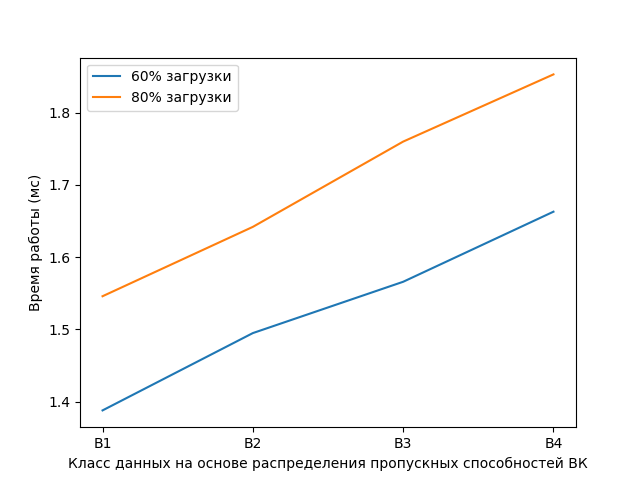
\includegraphics[width=0.60\textwidth]{img/double_res_sw.png}
	\caption{Работа алгоритма при выходе из строя коммутатора в топологии <<Двойное резервирование>>.}
	\label{pic:double_res_sw}
\end{figure}


На рисунках~\ref{pic:4node_res}--\ref{pic:double_res_sw} продемонстрирована работа алгоритмов на различных топологиях при возникновении отказов. Для топологии <<Ромб>> (см. рисунок~\ref{pic:4node}) не был рассмотрен случай выхода из строя коммутатора, так как такой отказ требует переноса задач между вычислителями, а этот процесс не рассматривается в рамках данной работы.

Назовем увеличением тяжести системы виртуальных каналов увеличение процентного содержания в ней виртуальных каналов с высокой пропускной способностью. Таким образом тяжесть системы виртуальных каналов увеличивается от класса~B1 к классу~B4. 

На загруженности сети 80\% алгоритм работает незначительно дольше, чем на загруженности 60\%. Исключение составляют случаи, в которых на низкой загрузке используется базовый этап алгоритма, а на высокой дополнительный. В этих случаях разница во времени работы на одном и том же классе данных более значительна.

Резкое увеличение времени работы алгоритма, отображенное на графиках, также связано с переходом к дополнительному этапу. На топологиях с большим количеством альтернативных путей время работы алгоритма возрастает сильнее при увеличении тяжести системы виртуальных каналов. Это демонстрируют результаты для топологии <<Ассиметрия>>. При этом на топологии <<Двойное резервирование>> рост времени работы практически не наблюдается из-за небольшого множества альтернативных маршрутов.

\FloatBarrier

\subsection{Апробация разработанного подхода к динамической реконфигурации сети} \label{subsec:approbation}
\subsubsection{Конфигурация экспериментальной системы}
Система апробации представляет собой виртуальную среду, имитирующую
функционирование:
\begin{enumerate}
	\item Контроллера сети.
	\item Набора коммутаторов.
	\item Абонентов сети, формирующих потоки данных с заданными характеристиками.
\end{enumerate}

Виртуальная среда разворачивается на основе операционной системы Linux Ubuntu 16.04,
на которой установлены следующие компоненты:
\begin{enumerate}
	\item Runos -- ПКС-контроллер \cite{runos}.
	\item Ofsoftswitch13 -- программный коммутатор, поддерживающий OpenFlow 1.3 \cite{ofsoftswitch}.
	\item Mininet -- средство, имитирующее работу сети \cite{mininet}.
\end{enumerate}

\subsubsection{Сценарии апробации}

Для апробации предложенного подхода к передаче данных в реальном времени был выбран набор сценариев, основывающийся на том, какие элементы сети могут выйти из строя. 

Рассматривается выход из строя:
\begin{enumerate}
	\item Коммутатора.
	\item Физической линии, соединяющей два коммутатора.
	\item Физической линии, соединяющей абонента с коммутатором.
	\item Порта абонента или коммутатора.
\end{enumerate}

Данные сценарии запускались на разных классах исходных данных по распределению пропускной способности и с загрузкой сети 80\%. 

Дополнительно к этому рассматриваются сценарии кратных последовательных во времени выходов из строя элементов сети. Последовательности отказов можно найти в таблице A3 в приложении A. Для таких сценариев рассматривались наборы виртуальных каналов с загрузкой 50\% и третьим классом данных по распределению пропускных способностей. Низкая начальная загрузка сети была выбрана так как последовательные разрывы требуют большего количества свободной пропускной способности.

Сценарии разрыва физической линии между коммутаторами и выхода из строя соответствующих портов выполняются на всех топологиях. Оставшиеся сценарии могут быть выполнены только на топологиях <<Двойное резервирование>> и <<Ассиметрия>> (см. рисунки~\ref{pic:double} и~\ref{pic:5node}). Отказ портов практически ничем не отличается от отказа соответствующих им физических линий. Поэтому в таблице результатов данные по таким сценариям представлены не будут.

\subsubsection{Методика апробации}
Апробация работы алгоритма реконфигурации в рамках предложенного подхода состоит из трёх этапов:
\begin{enumerate}
	\item Формирование набора тестовых прецедентов.
	\item Проведение экспериментов на тестовых прецедентах.
	\item Анализ результатов.
\end{enumerate}

Тестовые прецеденты формируются выбором:
\begin{itemize}
	\item сценария апробации;
	\item класса исходных данных с доступной для выбранного сценария топологией сети.
\end{itemize}

На этапе проведения экспериментов производится запуск каждого тестового прецедента:
\begin{enumerate}
	\item Формируется соответствующая классу данных конфигурация сети.
	\item Запускается приложение реконфигурации.
	\item Запускается виртуальная тестовая среда, имитирующая поведение сети.
	\item Запуск приложения инициирует построение начальных маршрутов виртуальных каналов.
	\item Запуск тестовой среды инициирует отправку и прием потоков данных абонентами, а также сбор статистики по этим потокам данных.
	\item Средствами тестовой среды запускается сценарий апробации.
	\item Соответствующий сценарию отказ инициирует запуск алгоритма реконфигурации.
	\item По завершении приложение выдаёт информацию о времени, затраченном на применение изменений в сети.
	\item Происходит сворачивание тестовой среды, инициирующее обработку собранной статистики по потокам данных.
\end{enumerate}

На этапе анализа результатов для каждого тестового прецедента:
\begin{enumerate}
	\item Проверяется факт восстановления трафика по завершении выполнения сценария.
	\item Анализируется время, затраченное на применение изменений в сети.
	\item Анализируется число потерянных в ходе реконфигурации пакетов.
	\item Задержки и джиттеры, полученные после завершения реконфигурации сравниваются с эталонными задержками, полученными в штатном режиме.
	\item Делается вывод об успешности работы приложения реконфигурации в рамках предложенного сценария.
\end{enumerate}

\subsubsection{Результаты}

Результаты апробации работы алгоритма в рамках приложения, реализующего подход к передаче данных в условиях реального времени в ПКС, приведены в приложении A (см. таблицу A2). Результаты апробации случаев кратных последовательных разрывов также отражены в приложении А в таблице A3.

Джиттеры и задержки потоков данных, виртуальные каналы которых участвовали в реконфигурации, восстанавливались после завершения реконфигурации. Джиттеры и задержки прочих потоков данных не изменялись вообще.

Максимальное время, затраченное на процесс реконфигурации, составляет add мс и удовлетворяет наложенным в разделе~\ref{subsec:limits} ограничениям. Потери пакетов составили add. При этом потоки, маршруты виртуальных каналов которых не проходили через отказавшие элементы, затронуты не были.

Таблица A2 также демонстрирует, что часто с увеличением времени работы алгоритма время генерации и отправки правил падает. Это объясняется тем, что более глубокий поиск позволяет минимизировать число изменений, которые необходимо провести в сети.
 
Неуспех при построении новых виртуальных каналов имел место на тех же классах данных, что и при исследовании свойств алгоритма.

Было проверено несколько сценариев кратного последовательного во времени выхода из строя элементов сети. Максимальное число последовательных отказов, после которых восстанавливалась работоспособность системы, составило 4. Неуспех при восстановлении работы сети после очередного отказа был обусловлен исключительно отсутствием путей между абонентами или нехваткой пропускной способности физических линий. Время работы алгоритма add.

\subsection{Выводы}
Проведенное экспериментальное исследование продемонстрировало, что:
\begin{itemize}
	\item основные характеристики алгоритма (время работы, объем изменений в сети) соответствуют ожидаемым;
	\item алгоритм успешно функционирует в рамках приложения реконфигурации, работающего в виртуальной среде, имитирующей сеть ПКС;
	\item сохраняются характеристики качества обслуживания абонентских потоков данных при реконфигурации сети с использованием предложенного алгоритма.
\end{itemize}

Исследование и апробация показали, что предложенный алгоритм реконфигурации виртуальных каналов способен работать в составе приложения, реализующего подход к передаче данных в реальном времени в ПКС. Алгоритм успешно осуществляет поиск новых маршрутов для виртуальных каналов при выходе из строя различных элементов сети. Апробация показала работоспособность разработанного приложения, осуществляющего функции реконфигурации и мониторинга, и реализованного в нем подхода. Время, затраченное на осуществление реконфигурации, не превосходит ограничений, установленных для существующих систем реального времени.

\section*{Заключение}
\addcontentsline{toc}{section}{Заключение}

В рамках данной работы были достигнуты следующие результаты:
\begin{enumerate}
	\item Разработан подход к использованию ПКС в составе вычислительных систем реального времени, основанный на ранее предложенной автором схеме управления трафиком в ПКС.
	\item Предложен алгоритм динамической реконфигурации систем виртуальных каналов, предназначенный для работы в условиях реального времени и являющийся частью разработанного подхода.
	\item Предложенный алгоритм реализован в рамках приложения для ПКС-контроллера RUNOS, которое осуществляет функции мониторинга сети и её реконфигурации при возникновении отказов. Приложение представляет собой комплексную реализацию разработанного подхода.
	\item С использованием созданного приложения выполнено экспериментальное исследование алгоритма, продемонстрировавшее его временные характеристики и их соответствие описанным в работе ограничениям реального времени.
	\item С использованием созданного приложения выполнена апробация предложенного подхода в экспериментальной системе, имитирующей поведение ПКС-сети. Апробация продемонстрировала, что подход может быть использован в условиях реального времени.
\end{enumerate}

Предложенный подход позволяет осуществлять динамическую реконфигурацию вычислительных систем реального времени при выходе из строя различных элементов системы или смене режимов работы. Характеристики качества обслуживания для потоков данных абонентов восстанавливаются по завершении реконфигурации. Время, затрачиваемое на процесс смены конфигурации, не превосходит допустимого времени простоя сети в ВС РВ. Можно выделить несколько направлений дальнейшего развития данного подхода:
\begin{itemize}
	\item Сопряжение разработанного алгоритма и приложения со средствами перераспределения задач между вычислителями при возникновении отказов в условиях реального времени.
	\item Разработка поведения системы при неуспехе в работе предложенного алгоритма реконфигурации. Такое поведение может быть основано на задании уровней критичности для виртуальных каналов.
\end{itemize}

\renewcommand{\bibname}{Список литературы}
\addcontentsline{toc}{section}{\bibname}
\bibliographystyle{unsrt}
\begin{thebibliography}{}
	\bibitem{afdx}
	AFDX / ARINC 664 Tutorial (1500-049) // Condor Engineering, Inc. -- 2005.
	\bibitem{fcaert}
	Fibre Channel Arbitrated Loop (FC-AL) // working draft proposal American National Standard for Information Technology. 1995. 98 p.
	\bibitem{sdn}
	Software-Defined Networking: The New Norm for Networks // Open Networking Foundation. -- 2012. [PDF] (https://www.opennetworking.org/images/stories/downloads/sdn-resources/white-papers/wp-sdn-newnorm.pdf)
	\bibitem{vlsdn}
	Balashov V., Kostenko V., Ermakova T. An SDN-based approach to design of onboard real-time networks // Modern Network Technologies, MoNeTec-2018. -- Moscow, 2018. -- P. 16-22.
	\bibitem{vdovin}
	Vdovin P. M., Kostenko V. A. Organizing message transmission in AFDX networks // Programming and Computer Software. -- 2017. -- Vol. 43, No 1. -- P. 1-12. [DOI] (https://link.springer.com/article/10.1134\%2FS0361768817010078).
	\bibitem{meter}
	Efimushkin, T. Ledovskikh, D. Korabelnikov, D. Iazykov. Perfomance assurance in Software-Defined Networks // « Intellect Telecom» JSC.
	\bibitem{openflow}
	ONF OpenFlow Switch Specification, Version1.3.0 [PDF] (https://www.opennetworking.org/images/stories/downloads/sdn-resources/onf-specifications/openflow/openflow-spec-v1.3.0.pdf)
	\bibitem{ofsoftswitch}
	CPqD F. Openflow 1.3 software switch [HTML] (http://www.cpqd.github.io/ofsoftswitch13/).
	\bibitem{fakevlsdn}
	Cevher S. et al. A Fault Tolerant Software Defined Networking Architecture for Integrated Modular Avionics // 37th Digital Avionics Systems Conference (DASC). -- IEEE, 2018. -- P. 1-9.
	\bibitem{alg1}
	Al Sheikh A. et al. Optimal design of virtual links in AFDX networks // Real-Time Systems. -- 2013. -- Т. 49. -- No 3. -- P. 308-336.
	\bibitem{alg2}
	Botero J. F. et al. Optimal mapping of virtual networks with hidden hops // Telecommunication Systems. -- 2012. -- Т. 51. -- №. 4. -- P. 273-28
	\bibitem{alg3}
	Chowdhury N. M. M. K., Rahman M. R., Boutaba R. Virtual network embedding with coordinated node and link mapping // IEEE INFOCOM 2009. -- IEEE, 2009. -- P. 783-791.
	\bibitem{vdovinalg}
	Вдовин П. М. Инструментальная система проектирования сетей AFDX // Труды Московского физико-технического института. -- 2015. -- Т. 7. -- №. 2. -- P. 131-137.
	\bibitem{algsdn}
	Khan S., Wahid A., Tanvir S. Comparative study of routing strategies in software defined networking //Proceedings of the 31st Annual ACM Symposium on Applied Computing. -- ACM, 2016. -- P. 696-702.
	\bibitem{dejkstra}
	Golden B. Shortest-path algorithms: A comparison // Operations Research. -- 1976. -- Т. 24. -- №. 6. -- P. 1164-1168.
	\bibitem{kshort}
	Yen J. Y. Finding the k shortest loopless paths in a network // Management Science. -- 1971. -- Т. 17. -- No 11. -- P. 712-716.
	\bibitem{monitor1}
	Ochoa Aday L., Cervelló Pastor C., Fernández Fernández A. Current trends of topology discovery in OpenFlow-based software defined networks. -- 2015.
	\bibitem{monitor2}
	Pakzad F. et al. Efficient topology discovery in software defined networks // 2014 8th International Conference on Signal Processing and Communication Systems (ICSPCS). -- IEEE, 2014. -- P. 1-8.
	\bibitem{cpp}
	Orozco J. D., Santos R. M. Real-Time Operating Systems and Programming Languages for Embedded Systems. // INTECH Open Access Publisher. -- 2012.
	\bibitem{nox}
	Gude N. NOX: towards an operating system for networks // ACM SIGCOMM Computer Communication Review. -- 2008. -- Т. 38. -- №. 3. -- P. 105-110.
	\bibitem{runos}
	Shalimov A. et al. The Runos OpenFlow Controller // Software Defined Networks (EWSDN), 2015 Fourth European Workshop on. -- IEEE, 2015. -- P. 103-104.
	\bibitem{mininet}
	Oliveira R. L. S. Using mininet for emulation and prototyping software-defined networks // Communications and Computing (COLCOM) -- 2014. -- P. 1-6
\end{thebibliography}


\section*{Приложение A. Результаты экспериментального исследования} \label{sec:results}
\addcontentsline{toc}{section}{Приложение A. Результаты экспериментального исследования}

\begin{longtable}[c]{|c|c|c|c|}
\caption*{Таблица A1. Результаты исследования алгоритма}
\\
	\hline
\multicolumn{2}{|c|}{Класс данных} & \multirow{2}{*}{\begin{tabular}[c]{@{}c@{}}Успешность \\ завершения\\ (этап)\end{tabular}} & \multirow{2}{*}{\begin{tabular}[c]{@{}c@{}}Время \\ работы\\ (мс)\end{tabular}} \\ \cline{1-2}
		\begin{tabular}[c]{@{}c@{}}Распределение\\ по тяжести\end{tabular} & \begin{tabular}[c]{@{}c@{}}Загруженность \\ сети (\%)\end{tabular} & & \\ \hline
		\endfirsthead
		%
		\endhead
		%
		\multicolumn{4}{|c|}{Топология <<Ромб>>. Отказ линии s3-s4.} \\ \hline
		B1 & 60 & Базовый & 0.659 \\ \hline
		B1 & 80 & Базовый & 0.711 \\ \hline
		B2 & 60 & Базовый & 0.837 \\ \hline
		B2 & 80 & Базовый & 0.921 \\ \hline
		B3 & 60 & Базовый & 0.914 \\ \hline
		B3 & 80 & Дополнительный & 3.977 \\ \hline
		B4 & 60 & Дополнительный & 4.005 \\ \hline
		B4 & 80 & Неуспех & -- \\ \hline
		\multicolumn{4}{|c|}{Топология <<Ассиметрия>>. Отказ линии s1-s5.} \\ \hline
		B1 & 60 & Базовый & 0.645 \\ \hline
		B1 & 80 & Базовый & 0.785 \\ \hline
		B2 & 60 & Базовый & 1.6 \\ \hline
		B2 & 80 & Базовый & 1.801 \\ \hline
		B3 & 60 & Базовый & 2.371 \\ \hline
		B3 & 80 & Базовый & 2.622 \\ \hline
		B4 & 60 & Дополнительный & 5.77 \\ \hline
		B4 & 80 & Неуспех & -- \\ \hline
		\multicolumn{4}{|c|}{Топология <<Двойное резервирование>>. Отказ линии s2-s3.} \\ \hline
		B1 & 60 & Базовый & 1.738 \\ \hline
		B1 & 80 & Базовый & 1.864 \\ \hline
		B2 & 60 & Базовый & 1.818 \\ \hline
		B2 & 80 & Базовый & 1.97 \\ \hline
		B3 & 60 & Базовый & 1.959 \\ \hline
		B3 & 80 & Базовый & 2.022 \\ \hline
		B4 & 60 & Дополнительный & 3.073 \\ \hline
		B4 & 80 & Неуспех & -- \\ \hline
		\multicolumn{4}{|c|}{Топология <<Двойное резервирование>>. Отказ коммутатора s2.} \\ \hline
		B1 & 60 & Базовый & 1.388 \\ \hline
		B1 & 80 & Базовый & 1.546 \\ \hline
		B2 & 60 & Базовый & 1.495 \\ \hline
		B2 & 80 & Базовый & 1.642 \\ \hline
		B3 & 60 & Базовый & 1.566 \\ \hline
		B3 & 80 & Базовый & 1.76 \\ \hline
		B4 & 60 & Базовый & 1.663 \\ \hline
		B4 & 80 & Базовый & 1.853 \\ \hline
		\multicolumn{4}{|c|}{Топология <<Ассиметрия>>. Отказ коммутатора s5.} \\ \hline
		B1 & 60 & Базовый & 1.013 \\ \hline
		B1 & 80 & Базовый & 1.704 \\ \hline
		B2 & 60 & Базовый & 1.053 \\ \hline
		B2 & 80 & Дополнительный & 4.715 \\ \hline
		B3 & 60 & Базовый & 1.25 \\ \hline
		B3 & 80 & Дополнительный & 5.198 \\ \hline
		B4 & 60 & Дополнительный & 4.033 \\ \hline
		B4 & 80 & Дополнительный & 6.028 \\ \hline
		
\end{longtable}


\begin{longtable}[h]{|c|c|c|c|c|}
	\caption*{Таблица A2. Результаты апробации подхода.}
	 \\
	\hline
	\begin{tabular}[c]{@{}c@{}}Распределение\\ виртуальных каналов\\ по тяжести\end{tabular} & \begin{tabular}[c]{@{}c@{}}Время\\ работы алгоритма\\ (мс)\end{tabular} & \begin{tabular}[c]{@{}c@{}}Время генерации и \\ отправки правил \\ (мс)\end{tabular} & \begin{tabular}[c]{@{}c@{}}Максимальное\\ число потеряных\\ пакетов\end{tabular} \\ \hline
	\endfirsthead
	%
	\endhead
	\multicolumn{4}{|c|}{Топология <<Ромб>>. Отказ линии s3-s4.} \\ \hline
	B1 & 0.711 & 2.161 & 2 \\ \hline
	B2 & 0.921 & 1.1 & 2 \\ \hline
	B3 & 3.977 & 0.874 & 4 \\ \hline
	\multicolumn{4}{|c|}{Топология <<Ассиметрия>>. Отказ линии s1-s5.} \\ \hline
	B1 & 0.785 & 2.32 & 3 \\ \hline
	B2 & 1.801 & 1.765 & 4 \\ \hline
	B3 & 2.622 & 1.393 & 6 \\ \hline
	\multicolumn{4}{|c|}{Топология <<Ассиметрия>>. Отказ коммутатора s5.} \\ \hline
	B1 & 1.704 & & \\ \hline
	B2 & 4.715 & & \\ \hline
	B3 & 5.198 & & \\ \hline
	B4 & 6.028 & & \\ \hline
	\multicolumn{4}{|c|}{Топология <<Двойное резервирование>>. Отказ коммутатора s2.} \\ \hline
	B1 & 1.546 & 0.847 & 3 \\ \hline
	B2 & 1.642 & 0.858 & 2 \\ \hline
	B3 & 1.76 & 0.822 & 2 \\ \hline
	B4 & 1.853 & 0.614 & 2 \\ \hline
	\multicolumn{4}{|c|}{Топология <<Двойное резервирование>>. Отказ линии h2-s2.} \\ \hline
	B1 & & & \\ \hline
	B2 & & & \\ \hline
	B3 & & & \\ \hline
	B4 & & & \\ \hline
\end{longtable}

\begin{longtable}[h]{|c|c|c|c|c|}
	\caption*{Таблица A3. Результаты апробации множественных отказов.}
	\\
	\hline
	\begin{tabular}[c]{@{}c@{}}Номер \\ отказа\end{tabular} & \begin{tabular}[c]{@{}c@{}}Отказавший элемент \\ сети\end{tabular} & \begin{tabular}[c]{@{}c@{}}Время реконфигурации \\ (мс)\end{tabular} & \begin{tabular}[c]{@{}c@{}}Максимальное\\ число потеряных\\ пакетов\end{tabular} \\ \hline
	\endfirsthead
	%
	\endhead
	\multicolumn{4}{|c|}{Топология <<Ромб>>.} \\ \hline
	B1 & Линия s1-s3 & & \\ \hline
	B2 & Линия s4-s3 & & \\ \hline
	\multicolumn{4}{|c|}{Топология <<Ассиметрия>>.} \\ \hline
	B1 & Линия s1-s5 & & \\ \hline
	B2 & Линия s4-s5 & & \\ \hline
	B3 & Линия s2-s3 & & \\ \hline
	\multicolumn{4}{|c|}{Топология <<Ассиметрия>>.} \\ \hline
	B1 & Линия s2-s5 & & \\ \hline
	B2 & Линия s3-s5 & & \\ \hline
	B3 & Линия s4-s5 & & \\ \hline
	B4 & Коммутатор s5 & & \\ \hline
	\multicolumn{4}{|c|}{Топология <<Двойное резервирование>>.} \\ \hline
	B1 & Линия s3-h3 & & \\ \hline
	B2 & Линия s2-h2 & & \\ \hline
	B3 & Линия s1-h4 & & \\ \hline
	B4 & Линия s4-h4 & & \\ \hline
	\multicolumn{4}{|c|}{Топология <<Двойное резервирование>>.} \\ \hline
	B1 & Линия s2-h1 & & \\ \hline
	B2 & Линия s1-h4 & & \\ \hline
	B3 & Коммутатор s3 & & \\ \hline
	
\end{longtable}


\end{document}